% One-page version: cover page + ONE page with the plot and the discussion paragraph.
% Needs plot_onepage.png in the same folder.

\documentclass[11pt]{article}

\usepackage[utf8]{inputenc}
\usepackage{geometry}
\geometry{letterpaper, margin=1in}
\usepackage{setspace}
\usepackage{amsmath}
\usepackage{amssymb}
\usepackage{graphicx}
\usepackage{xcolor}
\usepackage{fancyhdr}
\usepackage{hyperref}
\hypersetup{colorlinks=true, linkcolor=blue, urlcolor=blue, pdfborder={0 0 0}}
\pagestyle{fancy}
\fancyhf{}
\fancyfoot[C]{\thepage}

\newcommand{\hwNumber}{\#2}
\newcommand{\hwTitle}{Tuning a single note on your instrument}

\begin{document}

%% ------------------------- Cover page -------------------------
\begin{center}
    \vspace*{2cm}
    \textbf{Vanderbilt University \\}
    \textbf{School of Engineering \\}
    \vfill
    \textbf{ES 1402-13 \\}
    \textbf{Dr. Bellan\\}
    \textbf{Fall 2026-2027\\}
    \textbf{\today \\}
    \textbf{HW 2: \hwTitle \\}
    \vfill
    \textbf{Youssef Nassar \\}
    (Student ID: nassary) \\
    \vfill
\end{center}

\thispagestyle{empty}
\newpage
\pagenumbering{arabic}

\fancyhead[L]{\footnotesize\textbf{Vanderbilt University}}
\fancyhead[C]{\footnotesize\textbf{\hwTitle\ \hwNumber}}
\fancyhead[R]{\footnotesize\textbf{ES 1402}}

%% ------------------------- The one page -------------------------
\setstretch{1.12}

\begin{center}
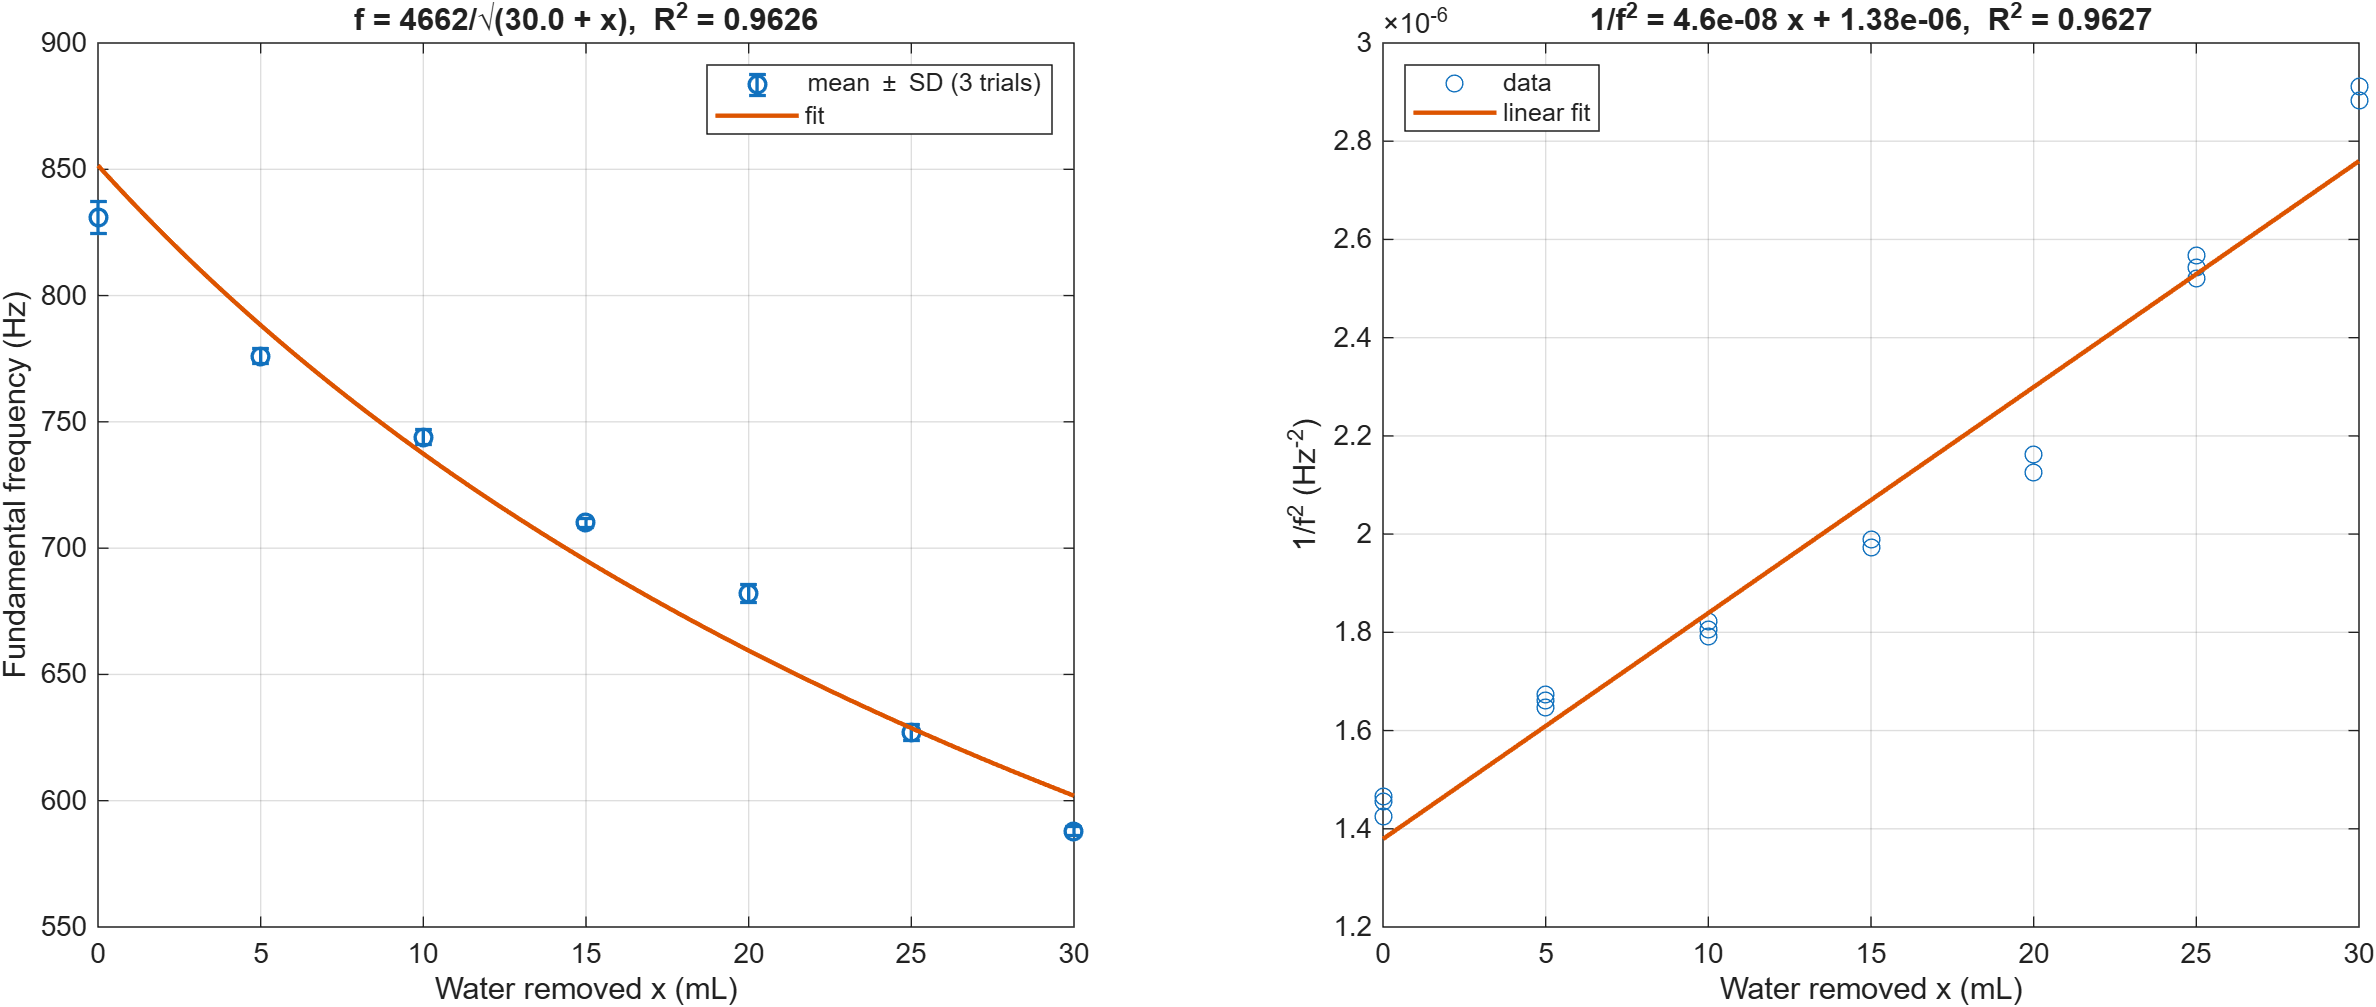
\includegraphics[width=\linewidth]{plot_onepage.png}\\[0.2em]
{\small\textbf{Figure 1.} Water-tuned Helmholtz bottle. Left: fundamental frequency (Friture) vs.\ water removed $x$, mean $\pm$ SD of 3 trials at each of 7 settings, with the fit $f = a/\sqrt{V_0 + x}$.
Right: linearized data, $1/f^2$ vs.\ $x$, with the straight-line fit.}
\end{center}

\vspace{0.4em}
\noindent
A Helmholtz-resonator bottle was built from a 355 mL Aquafina bottle containing 343 mL of water, which left 50 mL of air. When air is blown across the open neck, the plug of air in the neck
oscillates against the springiness of the air in the bottle, like a mass on a spring, and the tone is recorded in Friture. The note is tuned by removing water with a 60 mL syringe: the water removed, $x$,
increases the air volume $V = V_0 + x$, and more air gives a softer spring and a lower pitch (831 Hz at $x = 0$ to 588 Hz at $x = 30$ mL). The physical model is the Helmholtz resonance,
$f = \frac{c}{2\pi}\sqrt{A/(V L_\mathrm{eff})}$, with $L_\mathrm{eff} = L + 0.85\,d$, where $0.85\,d$ is the standard end correction for the air that moves just outside and inside the neck.
Since only $V$ is changed, $f \propto V^{-1/2}$, or equivalently $1/f^2 = (x + V_0)/a^2$ is linear in $x$, so a straight line was fitted to $1/f^2$ versus $x$.
The measurements were very repeatable (standard deviation 1.7--6.2 Hz, or 0.2--0.7\% of the frequency); the remaining scatter is most likely caused by small changes in blowing angle and lip position.
The fit gave $a = 4662$ (theory 5123, ratio 0.91), $V_0 = 30.0$ mL (expected $\approx 41$ mL, from 50 mL of air minus about 9 mL of air in the neck), and $R^2 = 0.963$, so the trend is captured but the fit is not perfect:
the residuals are systematic, because the $20\to25$ and $25\to30$ mL steps changed $1/f^2$ about twice as much as the earlier steps. When only $x \le 20$ mL was fitted, $a = 5381$ (ratio 1.05),
$V_0 = 42.4$ mL and $R^2 = 0.994$ were obtained, in good agreement with theory, which supports the model. The mismatch is therefore attributed to the last two settings, where more water was probably removed than
the syringe readings indicate (this was not confirmed), together with the approximate end correction and slight flexing of the thin bottle walls. All 7 points were kept.

\end{document}
